% !TeX root = ./lensing-lfi.tex

\documentclass[twocolumn]{aastex62}

\usepackage{amsmath, amsthm, amssymb, amsfonts}

\newcommand{\SM}[1]{{\bf \color{blue}{[SM: #1]}}}
\newcommand{\JB}[1]{{\bf \color{purple}{[JB: #1]}}}

\newcommand{\animicon}{\faPlayCircle}
\newcommand{\nbicon}{\faFileCodeO}

\newcommand{\animlink}[1]{\href{https://github.com/smsharma/StrongLensing-Inference/blob/master/figures/#1.gif}{\animicon}\xspace}
\newcommand{\nblink}[1]{\href{https://github.com/smsharma/StrongLensing-Inference/blob/master/notebooks/#1.ipynb}{\nbicon}\xspace}

\newcommand{\acronym}[1]{{\small{#1}}\xspace}
\newcommand{\package}[1]{\textsl{#1}\xspace}
\newcommand{\Euclid}{\textsl{Euclid}\xspace}
\newcommand{\lcdm}{$\Lambda$CDM\xspace}
\newcommand{\kpc}{\textrm{kpc}}
\newcommand{\Msun}{\textrm{M}_\odot}
\newcommand{\kmps}{\textrm{km\,s}^{-1}}
\newcommand{\zl}{z_l}
\newcommand{\zs}{z_s}
\newcommand{\sv}{\sigma_v}
\newcommand{\mtwo}{m_{200}}
\newcommand{\MMW}{M_\textrm{MW}}
\newcommand{\Mtwo}{M_{200}}
\newcommand{\ctwo}{c_{200}}
\newcommand{\rtwo}{r_{200}}
\newcommand{\Rtwo}{R_{200}}

\newcommand{\eg}{{e.\,g.}\xspace}
\newcommand{\ie}{{i.\,e.}\xspace}
\newcommand{\diff}{\mathrm{d}}
\newcommand{\overbar}[1]{\mkern 1.5mu\overline{\mkern-1.5mu#1\mkern-1.5mu}\mkern 1.5mu}
\newcommand{\fsub}{f_{\mathrm{sub}}}
\newcommand{\nsub}{n_{\mathrm{sub}}}
\newcommand{\pref}{p_{\mathrm{ref}}}
\newcommand{\stattheta}{\vartheta}
\newcommand{\mean}[1]{\makebox[0pt]{$\phantom{#1}\overline{\phantom{#1}}$}#1}

\DeclareMathOperator*{\argmin}{arg\,min}
\DeclareMathOperator{\pois}{Pois}
\DeclareMathOperator{\uniform}{Uniform}
\DeclareMathOperator{\normal}{\mathcal{N}\!}
\DeclareMathOperator{\expectation}{\mathbb{E}}
\DeclareMathOperator{\cov}{cov}
\DeclareMathOperator{\var}{var}



\shorttitle{Inferring dark matter substructure with machine learning}
\shortauthors{Brehmer and Mishra-Sharma et al.}
%@arxiver{}

\begin{document}\sloppy\sloppypar\raggedbottom\frenchspacing

\title{\textbf{%
Mining for Dark Matter Substructure: \\
Inferring subhalo population properties from strong lenses with machine learning
}}

\author{Johann Brehmer}
\affil{Center for Cosmology and Particle Physics, Department of Physics, New York University, 726~Broadway, New York, NY 10003, USA}
\affil{Center for Data Science, New York University, 60 Fifth Ave, New York, NY 10011, USA}

\author{Siddharth Mishra-Sharma}
\affil{Center for Cosmology and Particle Physics, Department of Physics, New York University, 726~Broadway, New York, NY 10003, USA}
\email{sm8383@nyu.edu}

\author{Joeri Hermans}
\affil{University of Li\`ege, Belgium}

\author{Gilles Louppe}
\affil{University of Li\`ege, Belgium}

\author{Kyle Cranmer}
\affil{Center for Cosmology and Particle Physics, Department of Physics, New York University, 726~Broadway, New York, NY 10003, USA}
\affil{Center for Data Science, New York University, 60 Fifth Ave, New York, NY 10011, USA}

\begin{abstract}\noindent
The subtle and unique imprint of dark matter substructure on extended arcs in galaxy-galaxy strong lenses contains a wealth of information about the properties and distribution of dark matter on small scales and, consequently, about the underlying particle physics. Teasing out this effect poses a significant challenge however due to the high dimensionality of the underlying latent space associated with a large number of dark matter subhalos. We apply recently-developed simulation-based techniques to the problem of substructure inference in galaxy-galaxy strong lenses. By leveraging additional information extracted from the simulator, these methods can be used to train neural networks to estimate likelihood ratios associated with population-level parameters characterizing the distribution of substructure. We show through proof-of-principle application to simulated data how these methods can provide an efficient and principled way to infer substructure properties by simultaneously analyzing the large lens samples deliverable by upcoming surveys such as LSST and \emph{Euclid}.
\end{abstract}

\keywords{%
strong gravitational lensing (1643)
---
gravitational lensing (670)
---
nonparametric inference (1903)
---
astrostatistics techniques (1886)
---
cosmology (343)
---
dark matter (353)
}

\tableofcontents{}

\section{Introduction}
\label{sec:intro}

Dark matter (DM) accounts for nearly a quarter of the energy budget of the Universe, and pinning down its fundamental nature and interactions is one of the most pressing problems in cosmology and particle physics today. Despite an organized effort to do so through terrestrial~\citep{2018PhRvL.121k1302A,2017PhRvL.119r1302C,2017PhRvL.118b1303A}, astrophysical~\citep{2017ApJ...834..110A,2018PhRvD..98l3004C,2018PhRvL.120j1101L}, and collider searches~\citep{2019arXiv190301400A,2017PhLB..769..520S}, no conclusive evidence of interactions between the Standard Model (SM) and dark matter exists to-date.

An alternative and complementary approach involves studying dark matter directly through its irreducible gravitational interactions. The concordance Cold Dark Matter (CDM) framework of non-relativistic, collisionless dark matter particles provides an excellent description of the observed distribution of matter on large scales. However, many well-motivated models predict deviations from CDM on smaller scales. Fundamental dark matter microphysical properties, such as its particle mass and self-interaction cross-section, can imprint themselves onto its macroscopic distribution in ways that can be probed by current and future experiments~\citep{2019arXiv190201055D}. As motivating examples, theories where dark matter has a significant free-streaming length would lead to a dearth of subhalos at lower masses ($\lesssim 10^9\,\mathrm{M}_\odot$)~\citep{1983ApJ...274..443B,2001ApJ...556...93B,astro-ph/0004381,0807.0622,1008.0992}, and self-interactions~\citep{1508.03339,1311.6524,1211.6426,1208.3026,1201.5892,1805.03203,1904.10539} or dissipative dynamics~\citep{1706.04195,1702.05482,1707.03829,1303.1521,1512.05349} in the dark sector would modify the structure of the inner core of subhalos as compared to CDM predictions.

There exist several avenues for probing the structure of dark matter on small scales. While the detection of ultrafaint dwarf galaxies through the study of stellar overdensities and kinematics~\citep{1503.02584,0706.2687,1503.02079} can be used to make statements about the underlying dark matter properties, theoretical uncertainties in the connection between stellar and halo masses~\citep{1804.03097} and the effect of baryons on the satellite galaxy population~\citep{1812.00044,1811.11791,1701.03792,1608.01849} pose a challenge. Furthermore, suppressed star-formation in smaller halos means that there exists a threshold ($\lesssim 10^8\,\mathrm{M}_\odot$) below which subhalos are expected to be mostly dark and devoid of stars~\citep{1992MNRAS.256P..43E,1611.02281,1607.03127}. This makes studying the imprints of gravitational interaction the \emph{only} viable avenue for probing substructure at smaller scales. In this spirit, the study of perturbations to the stellar phase-space distribution in cold stellar streams~\citep{1804.06854,astro-ph/9807243,1109.6022,1303.4342,1811.03631}, and in stellar fields in the disk and halo~\citep{1711.03554} have been proposed as methods to look for low-mass subhalos through their gravitational interactions in the Milky Way.

Complementary to the study of locally-induced gravitational effects, gravitational lensing has emerged as an important tool for studying the distribution of matter over a large range of scales. Locally, the use of time-domain astrometry has been proposed as a promising method to measure the distribution of local substructure through correlated, lens-induced motions on background celestial objects~\citep{2018JCAP...07..041V}. In the extragalactic regime, galaxy-scale strong lensing systems are a laboratory for studying substructure. The presence of flux-ratio anomalies in multiply-imaged quasar lenses has been used to infer the typical abundance of substructure within galaxy-scale lenses~\citep{2002ApJ...572...25D,2019arXiv190504182H,2002ApJ...572...25D}. Lensed images of extended sources have been used to find evidence for a handful of subhalos with masses $\gtrsim 10^8\,\mathrm{M}_\odot$~\citep{1601.01388,0910.0760,1201.3643}.

A complementary approach relies on probing the collective effect of sub-threshold (\emph{i.e}, not individually resolvable) subhalos on extended arcs in strongly lensed systems. A particular challenge here is the high dimensionality of the latent parameter space associated with the large number of subhalos and their (potentially covariant) individual as well as population properties, a consequence of which is the intractability of the likelihood of high-level substructure parameters conditional on the data. Methods based on summary statistics~\citep{1702.00009} and studying the amplitude of spatial fluctuations on different scales through power spectra~\citep{1403.2720,1809.00004,1707.04590,1806.07897,1808.03501,1710.03075,1506.01724} have been proposed as ways to reduce the dimensionality of the problem and enable substructure inference in a tractable way. Trans-dimensional techniques may also be able to efficiently map out the parameter space associated with multiple sub-threshold subhalos in these systems~\citep{1508.00662,1706.06111}. This class of methods is well-suited to studying dark matter substructure since they can be sensitive to the \emph{population} properties of low-mass subhalos in strongly lensed galaxies which are directly correlated with the underlying dark matter particle physics. Furthermore, near-future observatories like LSST~\citep{0912.0201,2019arXiv190201055D,1902.05141} and \Euclid~\citep{1001.0061} are expected to find tens of thousands of galaxy-galaxy strong lenses~\citep{2015ApJ...811...20C}, making substructure inference in these systems (and high-resolution followups on a subset) one of the key ways to investigate dark matter substructure and stress-test the Cold Dark Matter paradigm in the near future. This calls for methods that can efficiently analyze large samples of lensed images to infer the underlying substructure properties with minimal loss of information stemming from dimensional reduction.

In this paper we apply a powerful recently-developed class of techniques for simulation-based inference~\citep{1805.00013,1805.00020,1805.12244} to the problem of extracting high-level substructure properties from an ensemble of galaxy-galaxy strong lensing images. In contrast to traditional simulation-based (or ``likelihood-free'') approaches, these methods do not rely on summary statistics and instead leverage additional information extracted from the simulator in order to train neural networks that can be used to efficiently estimate the likelihood ratio. This provides an elegant bridge between machine learning and the ubiquitous likelihood ratio, which is provably the most powerful statistic for hypothesis testing~\citep{1933RSPTA.231..289N}.

This paper is organized as follows. In Sec.~\ref{sec:lensing-formalism} we briefly review the formalism of gravitational strong lensing and describe our simulation setup, including the assumptions we make about the population of lensed sources and host galaxies, the substructure population and observational parameters. In Sec.~\ref{sec:lfi-formalism} we describe the simulation-based analysis technique used and its particular application to the problem of mining substructure properties from an ensemble of extended lensed arcs. We show a proof-of-principle application of this method to simulated data in Sec.~\ref{sec:results} and comment on how these methods can be extended to more ``realistic'' scenarios in Sec.~\ref{sec:extensions}. We conclude in Sec.~\ref{sec:conclusions}.

\section{Strong lensing formalism and simulation set-up}
\label{sec:lensing-formalism}

In strong lensing systems, the background light emission source can in general be a point-like quasar or supernova, or a faint, extended ``blue'' galaxy. The former results in multiple localized images on the lens plane rather than extended arc-like images, providing the ability to probe substructure over a limited region on the lens plane. For this reason, we focus our method towards galaxy-galaxy lenses --- systems producing images with extended arcs --- since we aim to disentangle the collective effect of a population of subhalo perturbers over multiple images. Young, blue galaxies are ubiquitous in the redshift regime $z\gtrsim1$ and dominate the faint end of the galaxy luminosity function, resulting in a much larger deliverable sample of galaxy-galaxy strong lenses compared to quadruply- and doubly-imaged quasars/supernovae.

We now briefly review the basic strong lensing formalism before describing in turn the models for the background source, lensing galaxy and population parameters of the lens systems used in this study.

\subsection{Strong lensing formalism}

We briefly review here the mathematical formalism behind strong lensing. For more details see, \emph{e.g.},~\cite{2001astro.ph..2341K,1992grle.book.....S}. For a mass distribution with dimensionless projected surface mass density $\kappa(\mathbf{x})=\Sigma(\mathbf{x}) / \Sigma_{\mathrm{cr}}$, where $\Sigma_{\mathrm{cr}}\equiv \frac{1}{4 \pi G_N} \frac{D_{\mathrm{s}}}{D_{\mathrm{ls}} D_{\mathrm{l}}}$ the critical lensing surface density, the two-dimensional lensing potential is given by
\begin{equation}
\psi(\mathbf{x})=\frac{1}{\pi} \int \ln |\mathbf{x}-\mathbf{y}| \kappa(\mathbf{y}) d \mathbf{y}.
\end{equation}
The lensed position of the source can be determined through the lens equation,
\begin{equation}
\mathbf{u}=\mathbf{x}-\nabla \psi(\mathbf{x})
\end{equation}
where $\mathbf{u}$ is the position of the source and $\nabla \psi$ is typically referred to as the deflection, which we will denote as $\boldsymbol\phi$ for brevity. For an extended source brightness profile $f_\mathrm{src}$, the final lensed image can be obtained as the the source profile evaluated on the image plane,
\begin{equation}
f^\prime_\mathrm{src}(\mathbf x) = f_\mathrm{src}(\mathbf{x}-\nabla \psi(\mathbf{x})).
\end{equation}
For a spherically symmetric, the radial deflection field is given by
\begin{equation}
\phi_{r}(r)=\frac{2}{r} \int_{0}^{r}du\,u \kappa(u) =\frac{1}{\pi \Sigma_{\mathrm{cr}}} \frac{M_{\mathrm{cyl}}(r)}{r}
\end{equation}
where $M_{\mathrm{cyl}}(r)$ is the mass enclosed within a cylinder or radius $r$. Extension to the slightly more general case of elliptical symmetry is straightforward (see, \emph{e.g.},~\cite{2001astro.ph..2341K}).

\subsection{Background source}

We model the emission from background source galaxies using a S\'{e}rsic profile, with the surface brightness given by
\begin{equation}
f_\mathrm{src}(r)=f_{e} \exp \left\{-b_{n}\left[\left(\frac{r}{r_{e}}\right)^{1 / n}-1\right]\right\},
\end{equation}
where $r_e$ is the effective circular half-light radius, $n$ is the S\'{e}rsic index, and $b_n$ is a factor depending on $n$ that ensures that $r_e$ contains half the total intensity from the source galaxy, given by~\citep{1999A&A...352..447C}
\begin{align}
b_n \approx 2 n &- \frac{1}{3} + \frac{4}{405 n} + \frac{46}{25515 n^2} \nonumber \\ &+ \frac{131}{1148175 n^3} - \frac{2194697}{30690717750 n^4}. \nonumber
\end{align}

We assume $n=1$ for the source galaxies, corresponding to a flattened exponential profile and consistent with expectation for blue-type galaxies at the relevant redshifts. $f_{e}$ encodes the flux at half-light radius, which can be mapped onto the total flux (or magnitude) associated with a given galaxy.

The total unlensed magnitude $M$ (in a given band) of a galaxy can be mapped on to $f_{e}$ as follows. For a detector with zero-point magnitude $M_0$, which specifies the magnitude of a source giving 1 count\,s$^{-1}$ in expectation, by definition the total counts are given by $S_\mathrm{tot}=10^{0.4(M-M_0)}$. Requiring the half-light radius to contain half the expected counts, for $n=1$ we have the relation $f_{e} \approx 0.526\,t_\mathrm{exp}S_\mathrm{tot} /(2\pi r_e^2)$ in counts\,arcsec$^{-2}$, where $t_\mathrm{exp}$ is the exposure length.

Treatment of the other S\'{e}rsic parameters, in particular the total emission and half-light radius, in the context of population studies is described in Secs.~\ref{sec:observations} and~\ref{sec:populations} below.

\subsection{Lensing host galaxy}

Cosmological $N$-body simulations suggest that the dark matter distribution in structures at galactic scales can be well-described by a universal, spherically symmetric NFW profile. However, strong lensing probes a region of the host galaxy much smaller than the typical virial radii of galaxy-scale dark matter halo, and the mass budget here is dominated by the baryonic bulge component of the galaxy. Taking this into account, the total mass budget of the lensing host galaxy, being early-type, can be well describe by a singular isothermal ellipsoid (SIE) profile, known as the bulge-halo conspiracy since neither the dark matter nor the baryonic components are individually isothermal. The host profile is thus described as
\begin{equation}
\rho(x, y)=\frac{\sigma_{v}^{2}}{2 \pi G\left(x^{2} / q+q y^{2}\right)}
\label{eq:hostprofile}
\end{equation}
where $\sigma_{v}$ is the central 1-D velocity dispersion of the lens galaxy and $q$ is the ellipsoid axis ratio, with $q=1$ corresponding to a spherical profile. The Einstein radius for this profile, giving the characteristic lensing scale, is given by
\begin{equation}
\theta_{{E}}=4 \pi\left(\frac{\sigma_{v}}{c}\right)^{2} \frac{D_{l s}\left(z_{l}, z_{s}\right)}{D_{s}\left(z_{s}\right)}
\label{eq:siethetae}
\end{equation}
where $D_{ls}$ and $D_s$ are respectively the angular diameter distances from the source to the lens planes and from the source plane to the observer respectively.

The deflection field for the SIE profile is given by~\citep{2001astro.ph..2341K}
\begin{align}
\phi_{x} &=\frac{\theta_E q}{\sqrt{1-q^{2}}} \tan ^{-1}\left[\frac{\sqrt{1-q^{2}} x}{\psi}\right] \\
\phi_{y} &=\frac{\theta_E q}{\sqrt{1-q^{2}}} \tanh ^{-1}\left[\frac{\sqrt{1-q^{2}} y}{\psi+q^{2} }\right]
\end{align}
with $\psi \equiv \sqrt{x^2 q^2 + y^2}$.

Although the total galaxy mass (baryons + dark matter) describe the macro lensing field, for the purposes of describing substructure we require being able to map the measure properties of an SIE lens onto the properties of the host dark matter halo. To do this, we relate the central stellar velocity dispersion $\sigma_v$ to the mass $M_{200}$ of the host dark matter halo. \citet{2018ApJ...859...96Z} derived a tight correlation between $\sigma_v$ and $M_{200}$, modeled as
\begin{equation}
\log\left(\frac{M_{200}}{10^{12}\,\Msun}\right) = \alpha + \beta\left(\frac{\sigma_v}{100\,\kmps}\right)
\label{eq:sigma_v_M_200_relation}
\end{equation}
with $\alpha = 0.09$ and $\beta = 3.48$. % with a mean log-normal scatter of 0.13\,dex.
We model the host dark matter halo with a Navarro-Frenk-White (NFW) profile~\citep{1996ApJ...462..563N,1997ApJ...490..493N}

\begin{equation}
\rho(r)=\frac{\rho_{s}}{\left(r / r_{s}\right)\left(1+r / r_{s}\right)^{2}}
\label{eq:rhoNFW}
\end{equation}
where $\rho_s$ and $r_s$ are the scale density and scale radius, respectively. The halo virial mass $M_{200}$ describes the total mass contained with the virial radius $r_{200}$, defined as the radius within which the mean density is 200 times the critical density of the universe and related to the scale radius through the concentration parameter $c_{200} \equiv r_{200}/r_s$. Thus, an NFW halo is completely described by the parameters $\{M_{200}, c_{200}\}$. We use the concentration-mass relation from~\citet{2014MNRAS.442.2271S} assuming a log-normal distribution for $c_{200}$ around the median inferred value given by the relation with scatter 0.15\,dex.

The spherically-symmetric deflection for an NFW perturber is given by~\citep{2001astro.ph..2341K}
\begin{equation}
\phi_{r}=4 \kappa_{s} r_{s} \frac{\ln (x / 2)+\mathcal{F}(x)}{x}
\end{equation}
where $x = r/r_s, \kappa_s = \rho_s\,r_s/\Sigma_\mathrm{cr}$ with $\Sigma_\mathrm{cr}$ the critical surface density, and
\begin{equation}
\mathcal{F}(x)=\left\{\begin{array}{ll}{\frac{1}{\sqrt{x^{2}-1}} \tan ^{-1} \sqrt{x^{2}-1}} & {(x>1)} \\ {\frac{1}{\sqrt{1-x^{2}}} \tanh ^{-1} \sqrt{1-x^{2}}} & {(x<1)} \\ {1} & {(x=1).}\end{array}\right.
\label{eq:Fx}
\end{equation}

We described the population parameters we use to model the host velocity dispersion (and thus its Einstein radius and dark matter halo mass) in Secs.~\ref{sec:observations} and~\ref{sec:populations} below.

\subsection{Lensing substructure}

The ultimate goal of our method is to characterize the substructure population in strong lenses. Here we describe our procedure to model the substructure contribution to the lensing signal. Understanding the expected abundance of substructure in galaxies over a large range of epochs is complex undertaking and an active area of research. Properties of individual subhalos (such as their density profiles) as well as those that describe their population (such as the mass and spatial distribution) are strongly affected by their host environment, and accurately modeling all aspects of subhalo evolution and environment is beyond the scope of this paper. Instead, we use simple physically justifiable assumptions to model the substructure contributions in order to highlight the broad methodological points associated with the application of our method.

 \lcdm, often called the standard model of cosmology, predicts a scale-invariant power spectrum of primordial fluctuations and the existence of substrucure over a broad range of masses with equal contribution per logarithmic mass interval. We parameterize the distribution of subhalo masses $\mtwo$ in a given host halo of mass $\Mtwo$ --- the subhalo mass function --- as power law distribution:
\begin{equation}
\frac{M_{200,0}}{\Mtwo}\frac{dn}{d\mtwo} = \alpha\left(\frac{\mtwo}{m_{200, 0}}\right)^{\beta}
\label{eq:shmf}
\end{equation}
where $\alpha$ encodes the overall substructure abundance, with larger $\alpha$ corresponding to more substructure, and the slope $\beta$ encodes the relative contribution of subhalos at different masses, with more negative $\beta$ corresponding to a steeper slope with more low-mass subhalos. The normalization factors $m_{200, 0}$ and $M_{200, 0}$ are arbitrarily set to $10^9\,\Msun$ and the Milky Way mass $\MMW \simeq 1.1\times10^{12}\,\Msun$, respectively.

Theory and simulations within the framework of \lcdm~predict a slope $\beta\sim-0.9$, giving a nearly scale-invariant spectrum of subhalos, which we assume in our fiducial setup.

% We follow the specifications in~\citet{2016JCAP...09..047H} in order to set the overall fiducial abundance of subhalos, normalizing $\alpha$ to give 150 subhalos in expectation between $10^{8}\,\Msun$ and $10^{10}\,\Msun$ for a Milky Way-sized host halo.
We parameterize the overall subhalo abundance through the mass fraction contained in subhalos, $f_\mathrm{sub}$, defined as the fraction of the total dark matter halo mass contained in bound substructure in a given mass range. We have
\begin{equation}
f_\mathrm{sub} = \frac{\int_{m_\mathrm{200, min}}^{m_\mathrm{200, max}}d\mtwo\,\mtwo\,\frac{dn}{d\mtwo}}{M_\mathrm{200,host}}
\end{equation}
For a given $f_\mathrm{sub}$, $\beta$ and host halo mass $M_\mathrm{200,host}$, this can be used to determine $\alpha$ in Eq.~\ref{eq:shmf}. The linear scaling of the subhalo mass function with the host halo mass $\Mtwo$ in Eq.~\ref{eq:shmf} is additionally described in~\citet{2016MNRAS.457.1208H,2017MNRAS.469.1997D}. In our fiducial setups, we take the minimum mass $m_\mathrm{200, min} = 10^7\,\Msun$ and $m_\mathrm{200, min} = 0.01\,\,M_\mathrm{200,host}$~\citep{2017MNRAS.469.1997D,2018PhRvD..97l3002H}, and corresponding fiducial substructure fraction in this range of 5\%, roughly consistent with~\citet{2018PhRvD..97l3002H,2019arXiv190504182H,2002ApJ...572...25D} within our considered mass range.

With all parameters of the subhalo mass function specified, the total number $n_\mathrm{tot}$ of subhalos expected within the virial radius $\Rtwo$ of the host halo can be inferred as $\int_{m_\mathrm{200, min}}^{m_\mathrm{200, max}}d\mtwo\,\frac{dn}{d\mtwo}$. Strong lensing probes a region much smaller this scale --- the typical Einstein radii for the host deflector are much smaller than the virial radius of the host dark matter halos. In order to obtain the expected number of subhalos within the lensing observations region of interest, we scale the total number of subhalos obtained from the above procedure by the ratio of projected mass within our region of interest $\theta_\textrm{ROI}$ and the host halo mass $\Mtwo$ as follows. We assume the subhalos to be distributed in number density following the host NFW dark matter profile. In this case, the NFW enclosed mass function is $M_\mathrm{enc}(x) = \Mtwo(\ln(x/2) + \mathcal{F}(x))$~\citep{2001astro.ph..2341K}, where $x$ is the angular radius in units of the virial radius, $x\equiv \theta/\theta_{200}$ and $\mathcal{F}$ is given by Eq.~\ref{eq:Fx} above. The number of subhalos within our ROI is thus obtained as $n_\mathrm{ROI} = n_\mathrm{tot} (\ln(x_\mathrm{ROI}/2) + \mathcal{F}(x_\mathrm{ROI}))$. We conservatively take the lensing ROI to enclose a region of angular size twice the Einstein radius of the host halo, $\theta_\mathrm{ROI} = 2\theta_E$.

Since strong lensing probes the line-of-sight distribution of subhalos within the host, their projected spatial distribution is approximately uniform within the lensing ROI~\citep{2017MNRAS.469.1997D}. We thus distribute subhalos uniformly within our ROI. The density profile of subhalos is assumed to be NFW and given by Eq.~\ref{eq:rhoNFW}, with associated lensing properties as described and the concentration inferred from the relation modeled in~\citet{2014MNRAS.442.2271S}.

We finally emphasize that we do not intent to capture all of the intricacies of the subhalo distribution, such as the effects of baryonic physics, tidal distruption of subhalos in proximity to the center of the host and redshift evolution of host as well as substructure properties. Although our description can be extended to take these into account, their precise characterization and effect is still subject to large uncertainties, and our simple model above captures the essential physics for demonstration purposes.

\subsection{Observational considerations}
\label{sec:observations}

A noted above, our method is best-suited to analyzing a statistical sample of strong lenses to search for substructure, such as those that are expected to be obtained in the near future with optical telescopes like \Euclid~and LSST. Given the challenges associated with the precise characterization of such a sample at the present time, we describe here the observational characteristics we assume in order to build up training and testing samples to validate our inference techniques.

We largely follow the description in~\citet{2015ApJ...811...20C}, and use the associated \package{LensPop} package, to characterize our mock observations. In particular, we use the detector configuration for \Euclid, assuming a zero-point magnitude $m_\mathrm{AB} = 25.5$ in the single optical VIS passband, pixel size 0.1\,arcsec, a Gaussian point spread function (PSF) with FWHM 0.18\,arcsec, individual exposures with exposure time 1610\,s, an isotropic sky background with magnitude 22.8\,arcsec$^{-2}$ in the detector passband.

These properties, in particular the exposure, sky background and PSF shape are expected to vary somewhat across the lens sample. Additionally, a given region may be imaged by multiple exposures over a range of color bands. Although these variations can easily be incorporated into our analysis, modeling this is beyond the scope of this study. We briefly comment on how this information can be taken into account later.

\subsection{Population statistics of the lens and source samples}
\label{sec:populations}

The fact that the strong lens population is expected to be dominated by higher-redshift ($z\gtrsim1$) blue source galaxies lensed by intermediate-redshift ($z\sim 0.5$--$1$) elliptical galaxies presents significant challenges for quantifying the lens population obtainable with future observations. Specifically, planned ground-based surveys like LSST and space telescopes like \Euclid~present complementary challenges for delivering images of strong lensing systems suitable for substructure studies. LSST is expected to image in six bands, allowing efficient source selection and distinguishing source and lens emission, but at the cost of lower resolution by virtue of being a ground-based instrument. \Euclid~imaging is expected be much higher in resolution but with a single optical passband (VIS). Near-IR imaging from WFIRST may deliver a high-resolution, multi-wavelength dataset that is more suitable for substructure studies, although the lens and source populations may differ from those probed by optical telescopes.

% In light of these uncertainties, we limit the scope of the present study to developing a class of methods that can be adapted to the specifications of a galaxy-galaxy strong lensing population obtained with the next generation of optical, near-IR and radio telescopes. In particular, we confine ourselves to a setting where the main methodological points can be made without detailed modeling of the detector capabilities and the deliverable lensing dataset, which is outside of the scope of the current paper.

In light of these uncertainties, we confine ourselves to a setting where the main methodological points can be made without detailed modeling of the detector capabilities and the deliverable lensing dataset, which is outside of the scope of the current paper. For concreteness, we simulate a sample of lenses with a simplified subset of host galaxy properties consistent with those deliverable by \Euclid~as modeled by~\citet{2015ApJ...811...20C}. In particular, we assume spherical lenses, with ellipticity parameter $q=1$ in Eq.~\ref{eq:hostprofile}. We draw the central 1-D velocity dispersions $\sigma_v$ of host galaxies from a normal distribution with mean 225\,km\,s$^{-1}$ and standard deviation 50\,km\,s$^{-1}$. Equation~\ref{eq:sigma_v_M_200_relation} the results of~\citet{2018ApJ...859...96Z} are used to map the drawn $\sigma_v$ to a dark matter halo mass $\Mtwo$, and the host Einstein radius is analytically inferred with Eq.~\ref{eq:siethetae}.

We draw the lens redshifts $z_l$ from a log-normal distribution with mean 0.56 and scatter 0.25 dex, discarding lenses with $z_l > 1$ as these tend to have a small angular size over which substructure perturbations are relevant. The source offsets $\theta_x$ and $\theta_y$ are drawn from a normal distribution with zero mean and standard deviation 0.2. These are consistent with the lens sample generated from the \package{LensPop} code packaged with~\citet{2015ApJ...811...20C}.

\begin{figure*}[tbp]
\centering
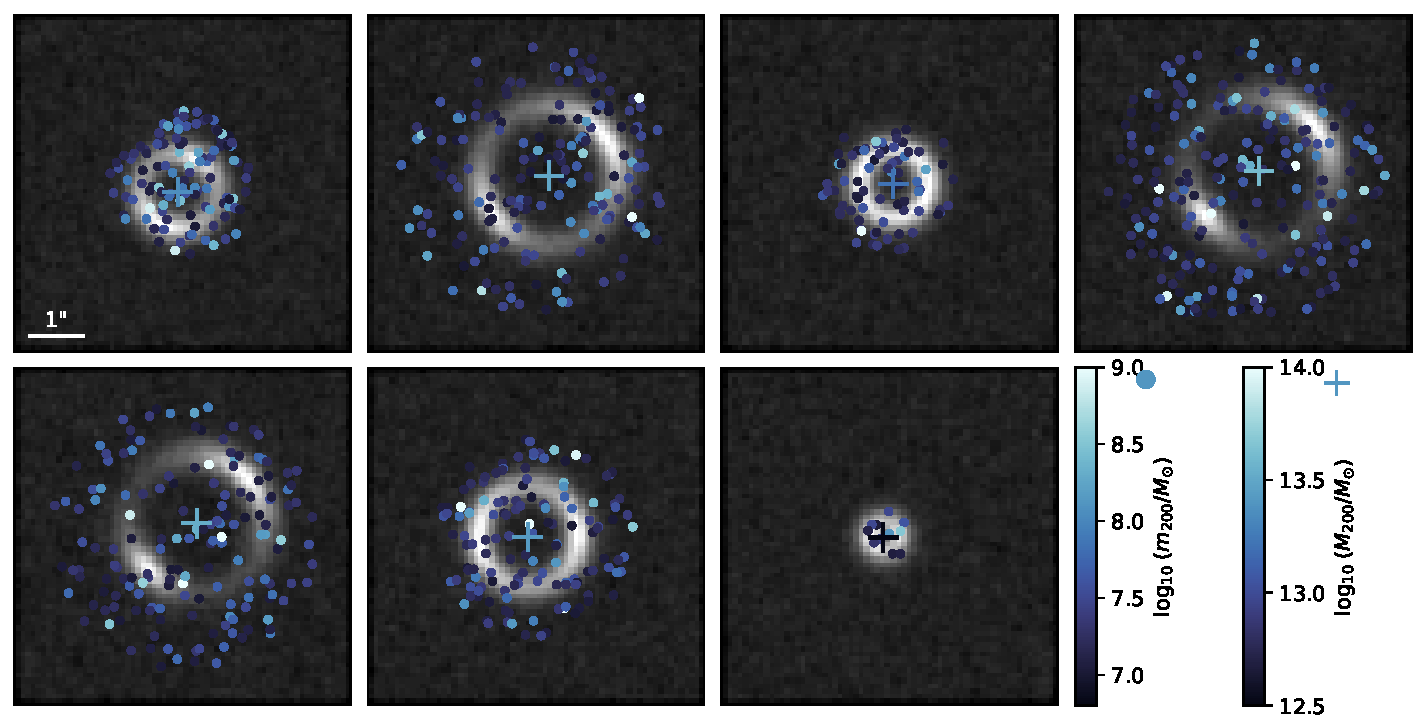
\includegraphics[width=1.\textwidth]{figures/simulations}
\caption{}
\label{fig:simulations}
\end{figure*}


\section{Statistical formalism and simulation-based inference}
\label{sec:lfi-formalism}

% % From introduction
% A complementary approach relies on probing the collective effect of sub-threshold (\emph{i.e}, not individually resolvable) subhalos on extended arcs in strongly lensed systems. A particular challenge here is the high dimensionality of the latent parameter space associated with the large number of subhalos and their (potentially covariant) individual as well as population properties, a consequence of which is the intractability of the likelihood of high-level substructure parameters conditional on the data. Methods based on summary statistics~\citep{1702.00009} and studying the amplitude of spatial fluctuations on different scales through power spectra~\citep{1403.2720,1809.00004,1707.04590,1806.07897,1808.03501,1710.03075,1506.01724} have been proposed as ways to reduce the dimensionality of the problem and enable substructure inference in a tractable way. Trans-dimensional techniques may also be able to efficiently map out the parameter space associated with multiple sub-threshold subhalos in these systems~\citep{1508.00662,1706.06111}. This class of methods is well-suited to studying dark matter substructure since they can be sensitive to the \emph{population} properties of low-mass subhalos in strongly lensed galaxies which are directly correlated with the underlying dark matter particle physics. Furthermore, near-future observatories like LSST~\citep{0912.0201,2019arXiv190201055D,1902.05141} and \Euclid~\citep{1001.0061} are expected to find tens of thousands of galaxy-galaxy strong lenses~\citep{2015ApJ...811...20C}, making substructure inference in these systems (and high-resolution followups on a subset) one of the key ways to investigate dark matter substructure and stress-test the Cold Dark Matter paradigm in the near future. This calls for methods that can efficiently analyze large samples of lensed images to infer the underlying substructure properties with minimal loss of information stemming from dimensional reduction.
%
% In this paper we apply a powerful recently-developed class of techniques for simulation-based inference~\citep{1805.00013,1805.00020,1805.12244} to the problem of extracting high-level substructure properties from an ensemble of galaxy-galaxy strong lensing images. In contrast to traditional simulation-based (or ``likelihood-free'') approaches, these methods do not rely on summary statistics and instead leverage additional information extracted from the simulator in order to train neural networks that can be used to efficiently estimate the likelihood ratio. This provides an elegant bridge between machine learning and the ubiquitous likelihood ratio, which is provably the most powerful statistic for hypothesis testing~\citep{1933RSPTA.231..289N}.

Our goal is to infer the subhalo mass function parameters from a catalog of images of observed lenses. In this section we will describe the challenges of this inference problem and our approach of simulation-based inference. For simplicity, we will use a more abstract notation, distinguishing between three sets of quantities in the lensing system:
%
\begin{description}
  \item[Parameters of interest $\theta$] The vector $\theta = (\fsub, \beta)^T$ parameterizes the subhalo mass function given, our goal is to infer their values.
  %
  \item[Latent variables $z$] A vector of all other unobservable random variables in the simulator. These include the mass and offset of the host galaxy, the number of subhalos in the region of interest, the position and mass of each subhalo, and the random variables related to the point spread function and Poisson fluctuations.
  %
  \item[Observables $x$] The observed lens images.
\end{description}

As described in the previous section, we have implemented a simulator for the lensing process in the ``forward'' direction: for given parameters $\theta$, the simulator samples latent variables $z$ and observed images $x, z \sim p(x, z|\theta)$. The joint likelihood of observables and latents $p(x, z|\theta)$ is schematically given by
%
\begin{multline}
  p(x,z | \theta)
  = p_{\mathrm{host}}(z_{\mathrm{host}}) \; \pois(n | \bar{n}_{\mathrm{ROI}}(\theta)) \\
   \prod_i^{n} \left[ p_m \left( m_{200, i} \middle| \theta \right) \; \uniform \left( r_i \right) \right] \\
  \times p_\mathrm{obs} \left( x \middle| f(z_{\mathrm{host}},\{(m_{200, i},r_i)\}) \right)
  \label{eq:joint_likelihood}
\end{multline}
%
where $p_{\mathrm{host}}$ summarizes the distribution of the host halo parameters $z_{\mathrm{host}}$ such as its mass, offset and redshift; $n$ is the actual number of subhalos in the region of interest,  $\bar{n}_{\mathrm{ROI}}( \fsub, \beta )$ is the mean number of subhalos in the region of interest as a function of the parameters $\theta = (\fsub, \beta)^T$; $m_{200, i}$ and $r_i$ are the subhalo masses and positions; $p_m(m) = 1/n \, \diff n / \diff m_{200}$ is the normalized subhalo mass function given in Eq.~\eqref{eq:shmf}; and in the last line $p_\mathrm{obs}$ is the probability of observing an image $x$ based on the true lensed image $f(z_{\mathrm{host}},\{(m_{200, i},r_i)\})$ due to the point spread function and Poisson fluctuations.

Inference with Markov Chain Monte Carlo (MCMC) methods based directly on this joint likelihood function $p(x,z | \theta)$ is feasible, but requires a large number of simulations for every observed lens. Instead, we use an approach that is based on the likelihood function of only the observables,
%
\begin{equation}
 p(x|\theta) = \int\!\diff z \; p(x, z|\theta) \,,
 \label{eq:likelihood_latent}
\end{equation}
%
where the latent variables are marginalised out. Being able to compute this likelihood function enables efficient frequentist and Bayesian inference. Unfortunately, even in our somewhat simplified simulator, each run of the simulation easily involves more than a thousand latent variables, and the integral over this enormeous space clearly cannot be computed explicitly. The likelihood function $p(x | \theta)$ is thus intractable, providing a major challenge for both frequentist and Bayesian inference.

This issue is often tackled by reducing the high-dimensional data $x$ to lower-dimensional summary statistics $v(x)$, for instance based on power spectra~\citep{1403.2720,1809.00004,1707.04590,1806.07897,1808.03501,1710.03075,1506.01724}. The likelihood $p(v|\theta)$ in the space of summary statistics can either be explicitly estimated through density estimation techniques such as histograms, kernel density estimation, or Gaussian processes, or replaced by a rejection probability in an Approximate Bayesian Computation (ABC) technique. While the compression to summary statistics makes the analysis tractable, it typically loses information and hence reduces the statistical power of the analysis.

We follow an alternative approach of simulation-based inference introduced in \citep{1805.00013,1805.00020,1805.12244}. It consists of four steps:
%
\begin{enumerate}
  \item During each run of the simulator, additional information that characterizes the subhalo population and lensing process is stored together with the simulated observed image.
  \item This information is used to train a neural network to approximate the likelihood ratio function.
  \item The neural network output is calibrated, ensuring that errors during training do not lead to wrong inference results.
  \item The calibrated network output is then used in either frequentist or Bayesian inference techniques.
\end{enumerate}

This approach enables amortized inference: after an upfront simulation and training phase, the neural network that estimates the likelihood ratio function can be evaluated very efficiently for any parameter point and observed image. Unlike MCMC based on the joint likelihood, this scales well to the expected large number of lenses expected in upcoming surveys.

In the remainder of this section, we will explain these four steps in detail.


\subsection{Extracting additional information from the simulator}
\label{sec:lfi-gold}

In a first step, we generate training data by simulating a large number of observed lenses. For each lens, we first draw two parameter point from a proposal distribution, $\theta, \theta' \sim \pi(\theta)$. This proposal distribution should cover the region of interest in the parameter space, but does not have to be identical to the prior in a Bayesian inference setting, which allows us to be agnostic about the inference setup at this stage.

Next, the simulator is run for the parameter point $\theta$, generating an observed image $x \sim p(x|\theta)$. In addition, we calculate and save two quantities: the joint likelihood ratio
%
\begin{equation}
  r(x,z | \theta) = \frac {p(x,z | \theta)} {p_\mathrm{ref}(x,z)}
  \equiv \frac {p(x,z | \theta)} {\int\!\diff\tilde{\theta} \, \pi(\tilde{\theta}) \, p(x,z | \tilde{\theta}) }
\end{equation}
%
and the joint score
%
\begin{equation}
  t(x, z | \theta) = \nabla_{\theta} \log p(x,z | \theta) \,.
\end{equation}
%
The joint likelihood ratio quantifies how much more or less likely a particular simulation chain including the latent variables $z$ is for the parameter point $\theta$ compared to a reference distribution. For this we choose the marginal distribution of latent variables and observables corresponding to the proposal distribution $\pi(\theta)$, which has support for every potential outcome of the simulation~\cite{Hermans:2019ioj}. The joint score is the gradient of the joint log likelihood in model parameter space and quantifies if a particular simulation chain becomes more or less likely with infinitesimal changes of the parameters of interest. Both quantities depend on the latent variables of the simulation chain.

We compute the joint likelihood ratio and joint score with Eq.~\eqref{eq:joint_likelihood}. Conveniently, many steps in the simulator do not explicitly depend on the parameters of interest $\theta$ and cancel in the joint likelihood ratio and joint score, and the remaining terms can be evaluated with little overhead to the simulation code. We also calculate the joint likelihood ratio $r(x,z|\theta')$ and the joint score $t(x,z|\theta')$ for the second parameter point $\theta'$ and store the parameter points $\theta$ and $\theta'$, the simulated image $x$, as well as the joint likelihood ratios and joint scores.

Our training samples consist of $10^6$ images, with parameter points chosen from a uniform range in $0.001 < \fsub < 0.2$ and $-1.5 < \beta < 0$.


\subsection{Machine learning}
\label{sec:lfi-ml}

How are the joint likelihood ratio and joint score, which are conditional on the latent variables $z$, useful to learn about the likelihood function $p(x|\theta)$, which only depends on the observed lens images and the parameters of interest? Consider the functional
%
\begin{multline}
  L[g(x, \theta)] = \int\!\diff\theta\! \int\!\diff\theta'\! \int\!\diff x\! \int\!\diff z \; \pi(\theta) \; \pi(\theta') \; p(x,z|\theta) \\
    \times \Biggl[
    - s \log g  - (1 - s) \log (1 - g) - s' \log g'  - (1 - s') \log (1 - g') \\
    + \alpha \Bigl\{ \left| t - \nabla_\theta \log \tfrac{1 - g}g \Bigr|_{\theta}  \right|^2
    + \left| t' - \nabla_\theta \log \tfrac{1 - g}g \Bigr|_{\theta'} \right|^2 \Bigr\}
   \Biggr]  \,,
   \label{eq:alices_loss}
\end{multline}
%
where we have abbreviated $s \equiv s(x,z|\theta) \equiv 1 / (1 + r(x,z|\theta))$,  $s' \equiv s(x,z|\theta') \equiv 1 / (1 + r(x,z|\theta'))$, $g \equiv g(x, \theta)$, $g' \equiv g(x, \theta')$, $t = t(x,z | \theta)$, and $t' \equiv t(x,z | \theta')$ for readability. Note that the test function $g(x, \theta)$ is a function of $x$ and $\theta$ only. In \citep{Stoye:2018ovl} it was shown that this modified cross-entropy or ``ALICES'' loss functional is minimized by the function
%
\begin{equation}
  g^*(x, \theta) \equiv \argmin_g L[g(x, \theta)] = \frac 1 {1 + r(x|\theta)} \,,
\end{equation}
%
one-to-one with the likelihood ratio function
%
\begin{align}
  r(x|\theta)
  &\equiv \frac {p(x|\theta)} {p_\mathrm{ref}(x)}
  \equiv \frac {p(x|\theta)} {\int\!\diff\tilde{\theta} \, \pi(\tilde{\theta}) \, p(x | \tilde{\theta}) } \notag \\
  &= \frac {1 - g^*(x, \theta)}{g^*(x, \theta)} \,.
\end{align}

This means that if we can construct the functional in Eq.~\eqref{eq:alices_loss} with the joint likelihood ratio and joint score extracted from the simulator and numerically minimize it, the resulting function lets us reconstruct the (otherwise intractable) likelihood function $r(x|\theta)$. Essentially, this step lets us integrate out the dependence on latent variables $z$ from the joint likelihood ratio and score, but in a general, functional form that does not depend on a set of observed images.

In practice, we implement this minimization with machine learning. A neural network plays the role of the test function $g(x, \theta)$, the integrals in Eq.~\eqref{eq:alices_loss} are approximated with a sum over training data sampled according to $\pi(\theta) \pi(\theta') p(x,z|\theta)$, and we minimize it numerically through a stochastic gradient descent algorithm. The neural network trained in this way provides an estimator $\hat{r}(x|\theta)$ of the likelihood ratio function that is exact in the limit of infinite training samples, sufficient network capacity, and efficient minimization. For a thorough discussion of this approach, we refer the reader to \cite{1805.00013,1805.00020,1805.12244,Stoye:2018ovl}.

Given the image nature of the lensing data, we choose a convolutional network architecture based on the ResNet-18~\cite{he2016deep} implementation in pyTorch~\cite{paszke2017automatic}. The parameters $\theta$ enter as additional inputs in the fully connected layers of the network. Compared to the original ResNet-18 architecture, we add another fully connected layer at the end to ensure that the relation between parameters of interest and image data can be modeled. All inputs are normalized to zero mean and unit variance. We train the networks over 100 epochs with a batch size of 128 with the Adam optimizer~\cite{}, exponentially decaying the learning rate from $3\cdot 10^{-4}$ to $3 \cdot 10^{-6}$, and use early stopping. This architecture and hyperparameter configuration performed best during a rough hyperparameter scan, though for this proof-of-concept study we have not performed an exhaustive optimization.


\subsection{Calibration}
\label{sec:lfi-calibration}

% 3: Calibration based on histograms. Comment on computational cost vs statistical guarantees.

\subsection{Inference}
\label{sec:lfi-inference}

% 4: Frequentist and Bayesian inference. Neyman-Pearson. Give posterior in terms of likelihood ratio estimator.


\section{Results}
\label{sec:results}

% \begin{figure*}[tbp]
% \centering
% \includegraphics[width=0.95\textwidth]{figures/placeholder}
% \caption{\SM{Placeholder for individual predictions}}
% \label{fig:profiles}
% \end{figure*}

% \begin{figure*}[tbp]
% \centering
% 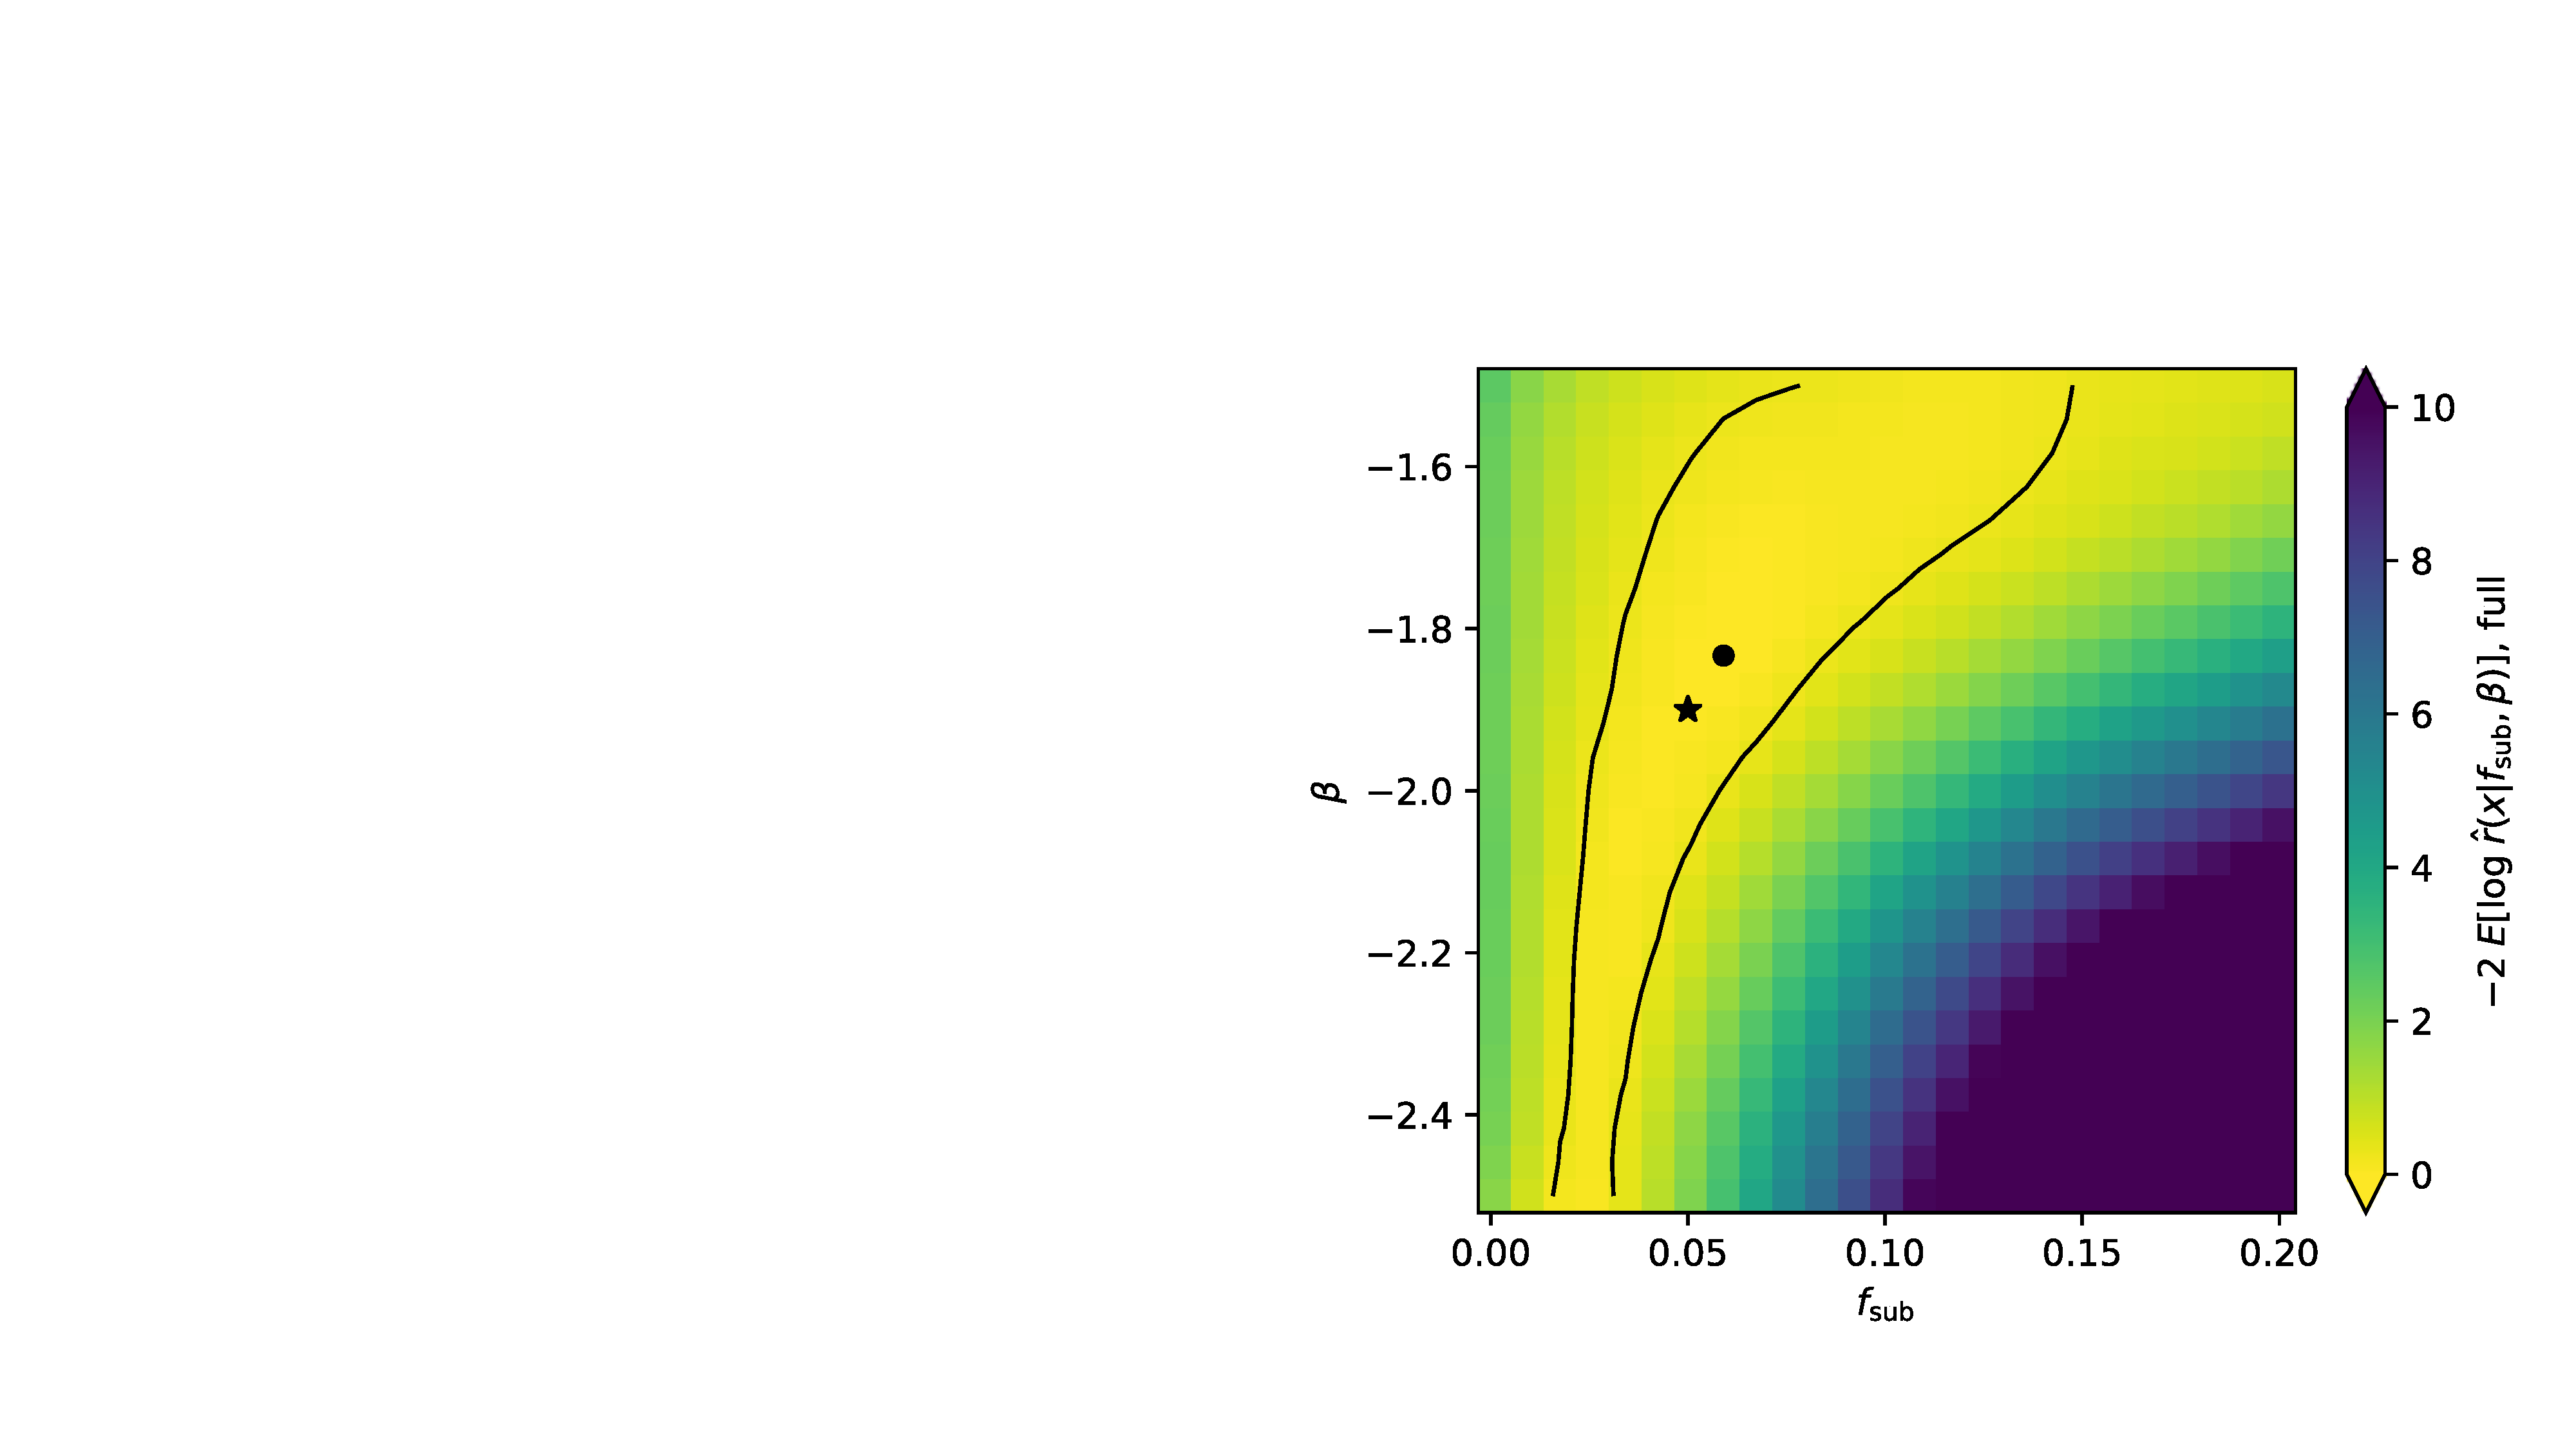
\includegraphics[width=0.45\textwidth]{figures/combined}
% 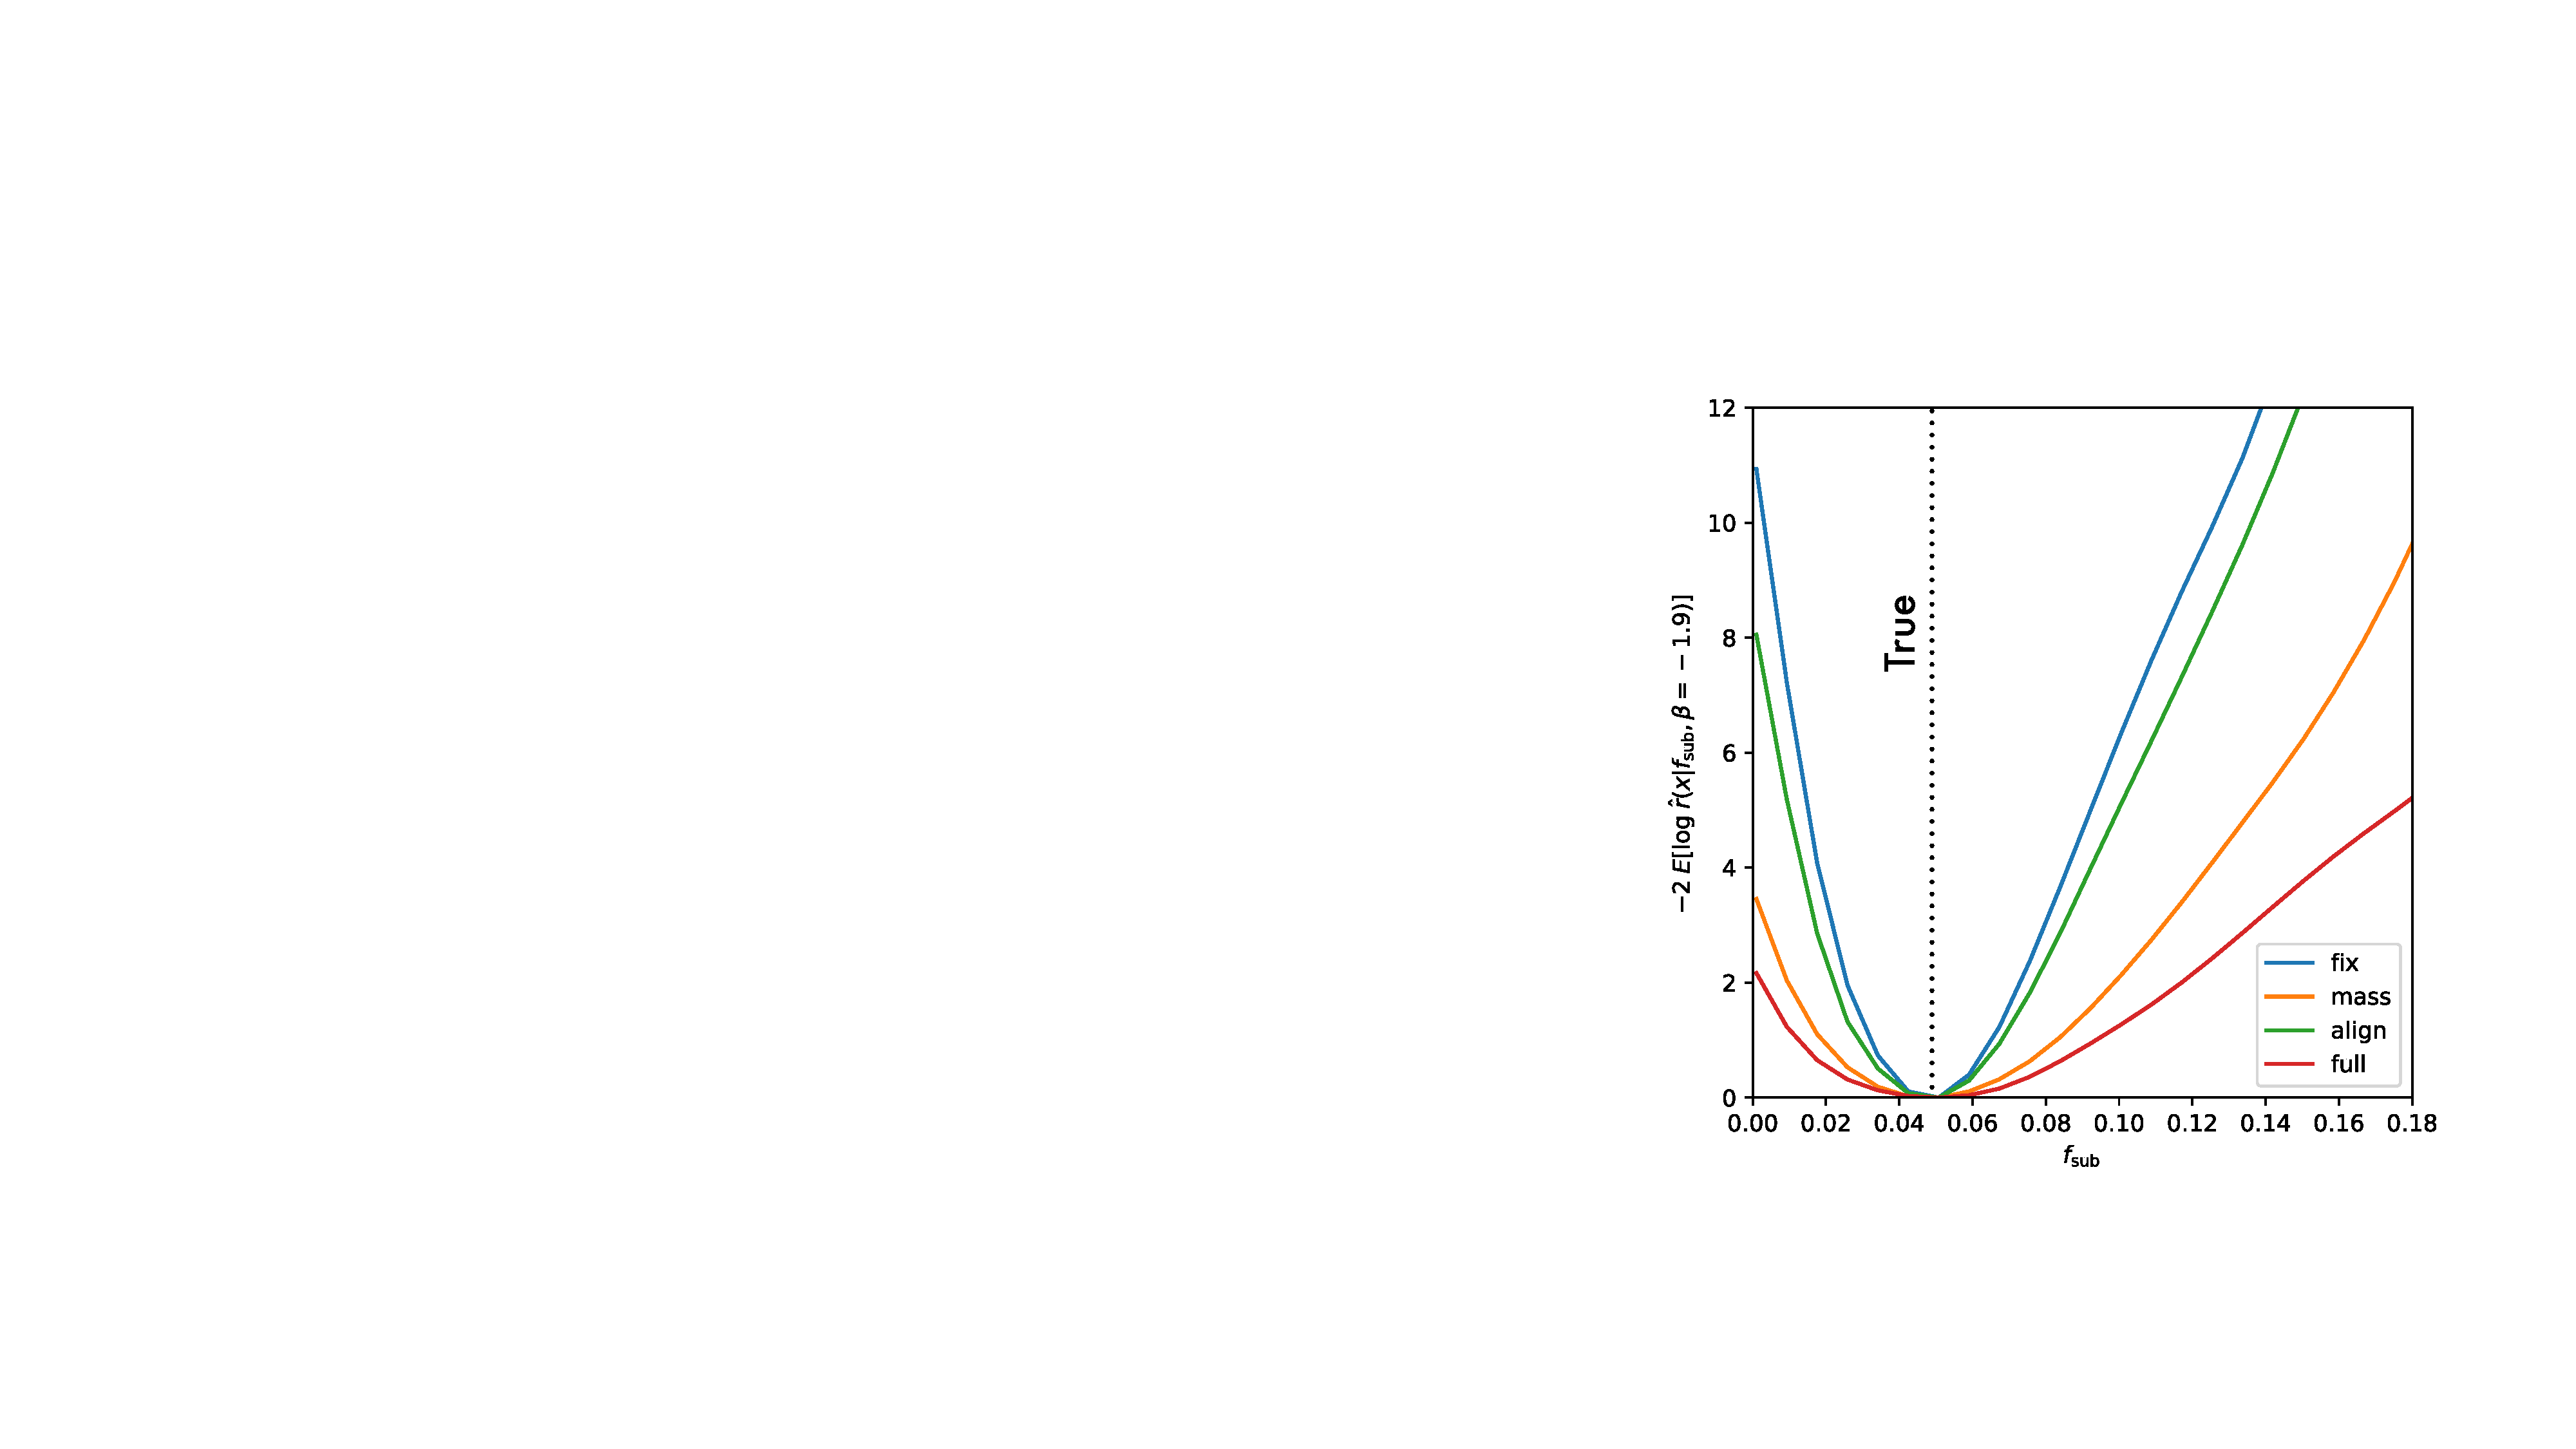
\includegraphics[width=0.35\textwidth]{figures/slices}
% \caption{}
% \label{fig:profiles}
% \end{figure*}

% \begin{figure*}[tbp]
% \centering
% 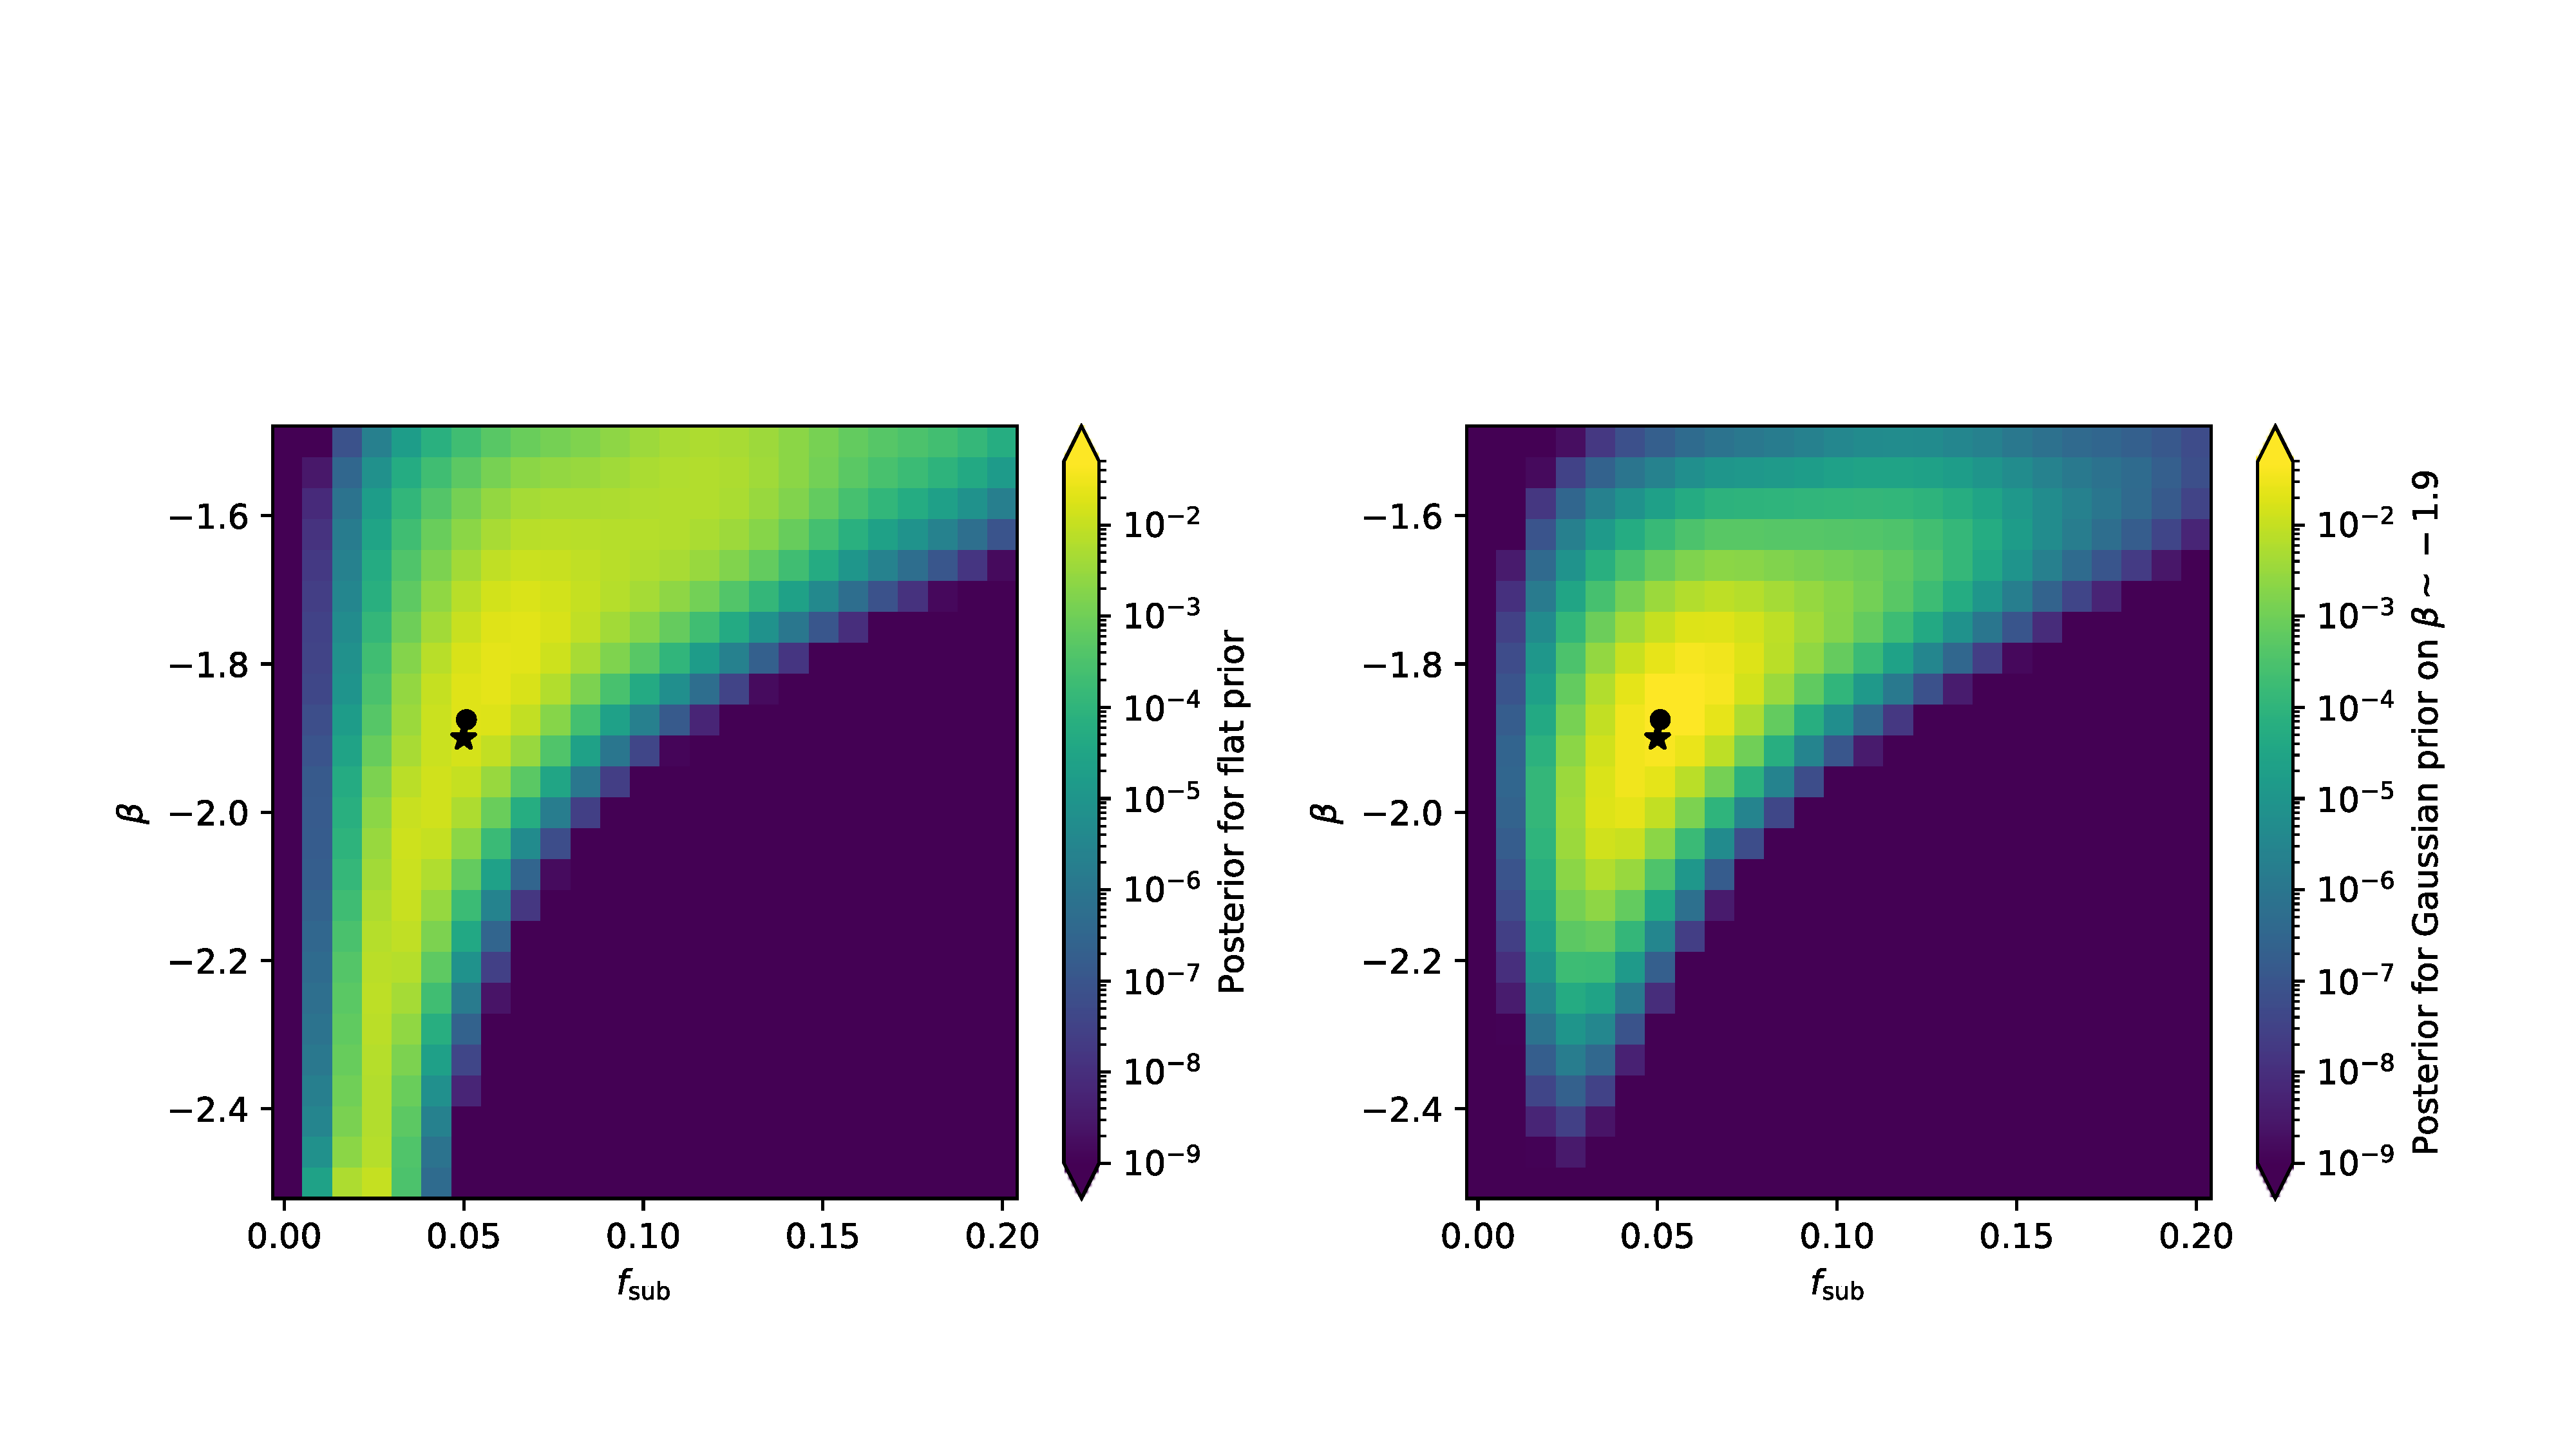
\includegraphics[width=1.\textwidth]{figures/bayesian}
% \caption{}
% \label{fig:bayesian}
% \end{figure*}

\section{Extensions}
\label{sec:extensions}

\section{Conclusions}
\label{sec:conclusions}

\acknowledgements
We thank Simon~Birrer, Christopher~Fassnacht, Daniel~Gilman, and Neal~Weiner for useful conversations. SM is partially supported by the NSF CAREER grant PHY-1554858 and NSF grant PHY-1620727.

\software{
\package{Astropy} \citep{2013A&A...558A..33A,2018AJ....156..123A},
\package{IPython} \citep{PER-GRA:2007},
\package{LensPop} \citep{2015ApJ...811...20C},
\package{MadMiner} \citep{Brehmer:2019xox},
\package{matplotlib} \citep{Hunter:2007},
\package{NumPy} \citep{numpy:2011},
\package{PyTorch} \citep{paszke2017automatic},
\package{SciPy} \citep{Jones:2001ab}.
}

\bibliographystyle{aasjournal}
\bibliography{lensing-lfi}

\end{document}
